\section{Feature Extraction and Per-pixel Classification}
\label{sec: Classification}

In this section, we describe the main classification algorithm used in the system. At each frame, the system looks at the depth image, and predicts each pixel's type of gestures (e.g., open hand, close hand or background). The prediction result on every pixel will be fed into a pooling stage to propose the final gesture location and type. The driving reason for us to choose per-pixel classification is that it allows massive parallelism using GPU since each pixel is using the same predicting algorithm.  

\subsection{Feature Extractions}
\label{sec: feacture_extraction}
For each pixel \textbf{x}, we extract a group of features. Each group say $\theta=\{\bf{u}, \bf{v} \}$ corresponds to the depth difference between two points offset from \textbf{x} normalized by its depth:

\begin{align} 
\label{eqn:feature}
f_{\theta}(x) = d\left(\textbf{x} + \frac{\textbf{u}}{d(\textbf{x})}\right) - d\left(\textbf{x} + \frac{\textbf{v}}{d(\textbf{x})}\right)
\end{align}

\begin{figure}
	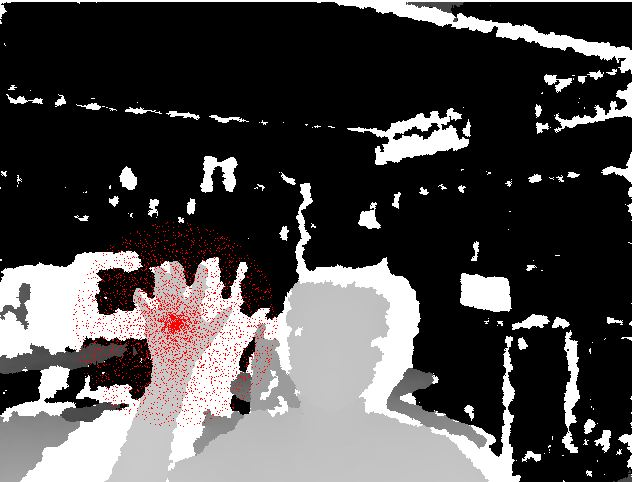
\includegraphics[width=0.23\textwidth]{fig/OpenHandNearOffset.jpg}
	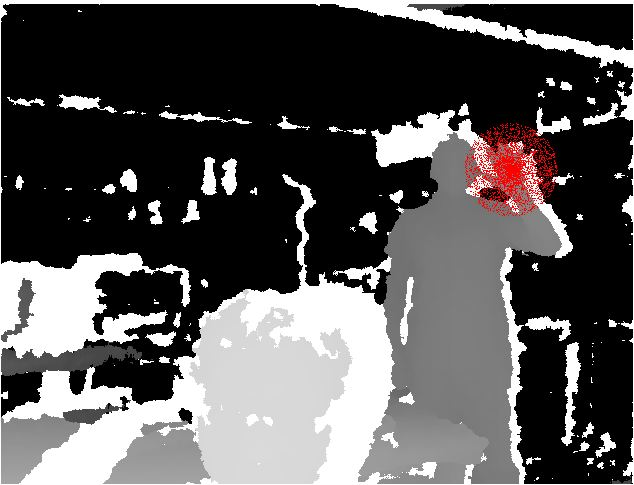
\includegraphics[width=0.23\textwidth]{fig/OpenHandFarOffset.jpg}
	
	\caption{Offset pairs for a given pixel. In the left figure, the reference pixel is the center of the palm. In the right figure, the reference pixel is the center of the palm of the person that stands. }
	\label{fig:offset}
\end{figure}

This feature extraction method is also used in \cite{shotton2011}. The offsets $\theta=\{\bf{u}, \bf{v} \}$ are generated randomly. In our design, we make those offsets to be uniformly sampled from a bounded circular area.  
$\textbf{u}$ and $\textbf{v}$ are obtained as
\begin{align}
\label{enq: offest}
 (r \cos \beta, r \sin \beta),
\end{align}
where $r$ and $\beta$ are uniform random variables:
\begin{align}
 r &= U[R_{\text{min}}, R_{\text{min}}] \\
 \beta &= U[0, 2\pi]
\end{align}

 As we can see from Figure \ref{fig:offset}, the offset pairs are located within the neighborhood of the palm and is adaptive to the depth.  
\todo{DO WE NEED MORE EXPLANATION?}

\subsection{The Classifier: SVM or Random Forest?}

In the training samples each pixel is labeled (we would deal with how to generate massive labeled sample in Section \ref{sec: generating_training}   and we have to use a supervised learning methods. Two methods come into our decision of choice: linear SVM and random forest. Let us make the notation as follows: the number of training samples: $l$, the number of features: $n$, the number of classes (types of gestures): $c$. Our main criteria for choosing the best algorithm are (1) prediction time and (2) accuracy. 

\textbf{Linear SVM.} In linear SVM, a model that is $c$ number of weight vector length of $n$ is trained. In prediction, the prediction is based on the dot product between the trained weight vectors and the feature vector. Therefore,  the run-time complexity for predicting each pixel is $O(n\times c)$.



\textbf{Random Forest.} Random forest is built on an ensemble of decision trees that are trained on  bootstrap\footnote{Bootstrap means uniform   sampling with replacement} samples of the training sets. The decision tree in the random forest is a binary tree. Each node in the decision tree has one feature and a threshold to determine which branch to go to by comparing the feature value to the threshold. In the leafs of the tree are labels. The final prediction is made by the majority rule of the all decision trees in the forest. More details about the training and statistical analysis can be seen in \todo{Random Forest paper}. The depth of the decision tree is approximately as $O(\log l)$. Therefore $O(\log l)$ queries of features are made in a single decision tree when prediction. The run-time complexity for making prediction in random forest is then $O(\log l \times n_{\text{tree}})$. In fact, we can prune each decision tree to limit its depth. Pruning is crucial for us since it can guarantee the \textbf{worst-case} prediction time. Moreover pruning can make the decision tree (which is a binary tree) almost balanced, ensuring the per-pixel prediction are done in almost constant time. Let us denote the maximum depth to be  $d_{\text{tree}}$, the run-time complexity can go down to $O(d_{\text{tree}}\times n_{\text{tree}})$. 

\todo{Show RF algorithm}

\textbf{Comparison.} Let us do a simple calculation in which we use a realistic parameter setting. Suppose we have 2000 features, 3 classes, and using 3 trees with maximum depth of 20, the random forest is 100 times faster than linear SVM! Moreover, in our experimental evaluation, random forest has proven to be far superior than linear SVM in accuracy. Although linear SVM might use some advanced feature learning technique such as deep learning to achieve similar accuracy as to random forest, SVM is still too slow for us to adopt in the system. Inheriting from decision tree, random forest allows the system to extract features \textbf{on-demand}, which has been extremely crucial for real-time application as in the case of our system. The second author \todo{HOW ABOUT THE FIRST AUTHOR? He's never surprised} is really surprised by this analysis since he used to believe linear SVM is unbeatable in practice.  

\textbf{Training.} Training in linear SVM can be very fast as it can has a run-time complexity of $O(n\times l)$ and there exists technique to scale the training to distributed system \todo{Cite Michael's paper}. Training in random forest, however, does not have an optimization-based foundation. We use brute force to determine the right feature and right threshold for each node in the decision forest. In determining the right threshold, we use grid search. In the training of random forest, it is highly recommended to put the training data in the main memory. 


\subsubsection{GPU For Real-time Prediction} 
There are $307,200$ $(640\times 480)$ pixels in a frame. Each pixel will undertake $O(d_{\text{tree}}\times n_{\text{tree}})$ operations for prediction. We first tried to implement the random forest prediction using CPU. It takes about 1 minute to process a frame! GPU has to be used since it allows massive parallelism. As can be seen in Figure~\ref{fig: GPUvsCPU}, GPU is more suitable for high-parallelism and high-latency jobs, while CPU is better fit for low-parallelism and low-latency jobs. 

\begin{figure}
	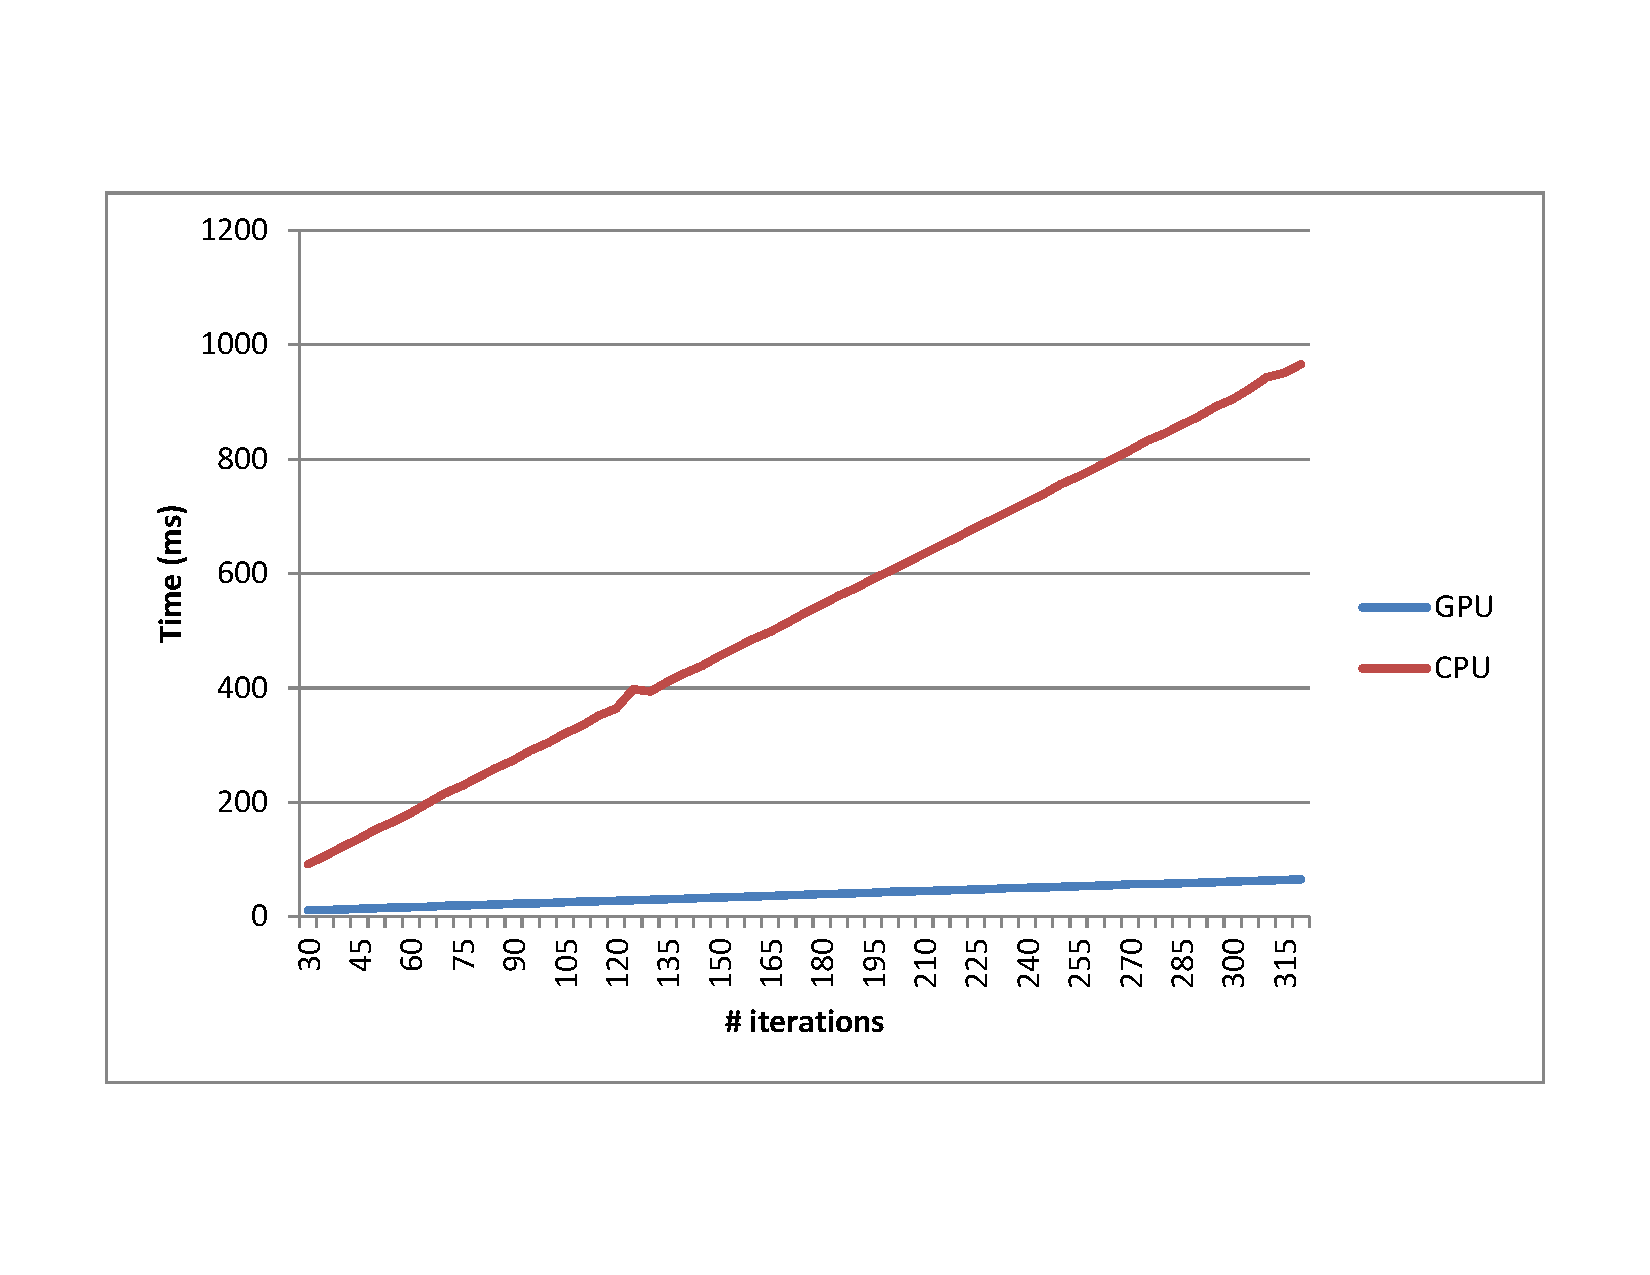
\includegraphics[width=0.45 \textwidth]{fig/GPUvsCPU.pdf}   
    \caption{A computational comparison between GPU and CPU. A simple experiment is conducted by varying the number of iterations in a for-loop. GPU would parallelize the for loop.}
    \label{fig: GPUvsCPU}
\end{figure}

In our system, each pixel has fired a thread to make prediction using random forest. In a typical GPU, more than thousands of threads are running concurrently thanks to the special architecture of GPU. As a result, per-pixel classification can be done in about 40ms \todo{Exact number}.    
